\documentclass[12pt,a4paper]{article} \usepackage[utf8]{inputenc} \usepackage[T1]{fontenc} \usepackage[brazil]{babel} \usepackage{graphicx} \usepackage{listings} \usepackage{xcolor} \usepackage{geometry} \geometry{margin=2.5cm} \lstset{ basicstyle=\ttfamily\footnotesize, keywordstyle=\color{blue}\bfseries, commentstyle=\color{green!50!black}, stringstyle=\color{red!60!black}, numbers=left, numberstyle=\tiny, stepnumber=1, numbersep=10pt, frame=single, breaklines=true, tabsize=4 } \title{Relatório de Laboratório – Lab 04 \\ Redes de Computadores e Internet} \author{Samuel Abrahão} \date{Faculdade IDP – 2025} \begin{document} \maketitle \section{Introdução} Neste relatório apresentamos a implementação de um sistema de comunicação simples baseado no protocolo UDP (User Datagram Protocol). O objetivo principal do laboratório é explorar o funcionamento de sockets em Python, compreender a natureza do tráfego sem conexão característico do UDP, e aplicar conceitos de codificação de dados utilizando o padrão Base64. Para tornar a análise mais robusta, foram utilizados experimentos de captura de pacotes, observação das mensagens enviadas e recebidas, bem como a execução de comandos de rede (\texttt{netstat}) para evidenciar a utilização das portas de transporte. \section{Fundamentação Teórica} O protocolo UDP é um dos principais protocolos de transporte da pilha TCP/IP. Ao contrário do TCP, o UDP não estabelece uma conexão antes da troca de dados, o que o torna um protocolo \textbf{não orientado a conexão}. Suas principais características incluem: \begin{itemize} \item Simplicidade na implementação; \item Menor sobrecarga, já que não possui mecanismos de confirmação e retransmissão; \item Adequado para aplicações em que velocidade é mais importante que confiabilidade absoluta (ex: streaming, VoIP, DNS). \end{itemize} No contexto deste laboratório, a simplicidade do UDP é explorada para enviar mensagens entre cliente e servidor sem necessidade de estabelecer conexões persistentes. Adicionalmente, aplicamos a codificação \textbf{Base64}, que converte uma cadeia de bytes em caracteres ASCII seguros para transmissão em protocolos que não toleram bytes arbitrários. Isso é bastante comum em e-mails, armazenamento de dados binários em formatos de texto, e transmissão em APIs. \section{Mensagens Enviadas e Recebidas} O cliente envia uma mensagem em texto puro (UTF-8). O servidor recebe essa mensagem, converte para Base64 e a retorna ao cliente. A seguir, apresentamos capturas de tela do processo: \subsection{Mensagem enviada (texto cru)} \begin{center} 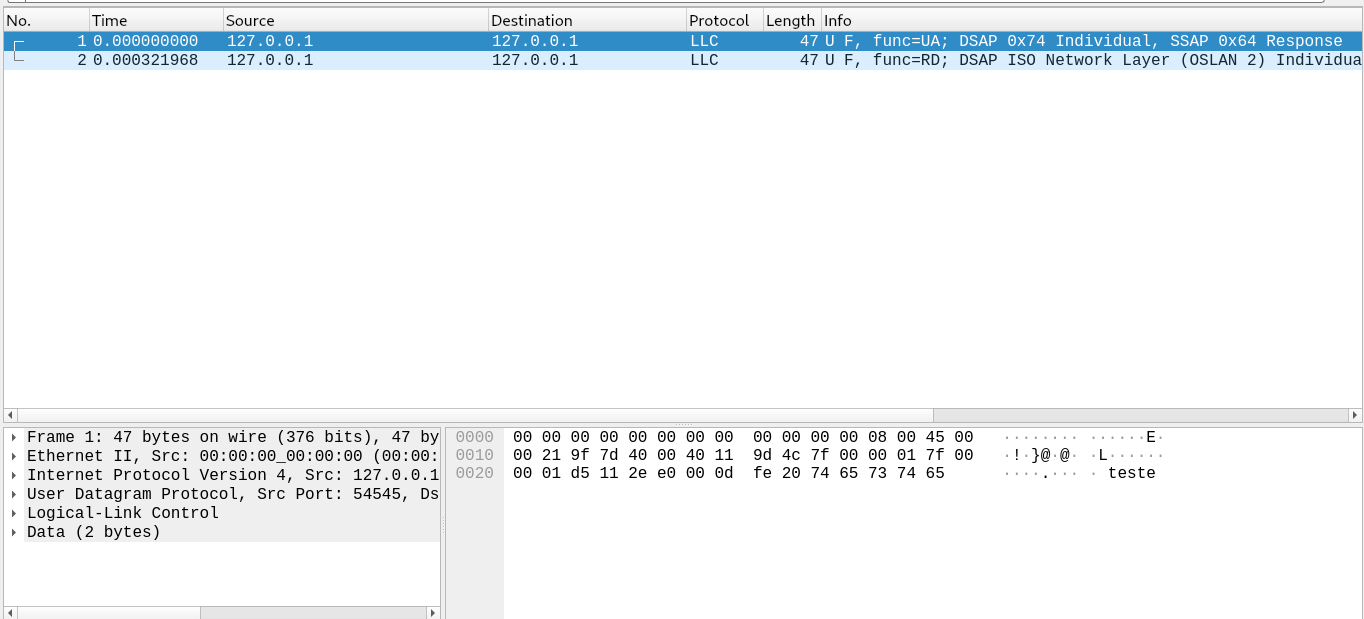
\includegraphics[width=0.7\textwidth]{assets/mensagemEnviadaCrua.png} \end{center} \subsection{Mensagem recebida pelo servidor (em Base64)} \begin{center} 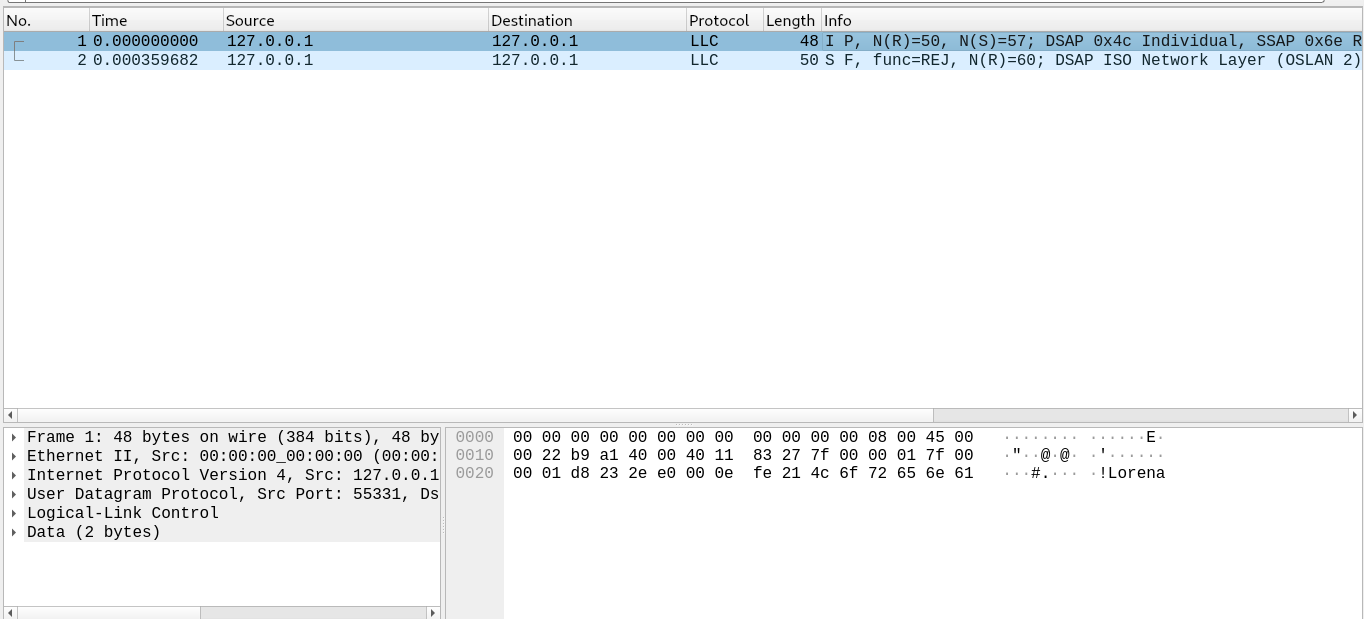
\includegraphics[width=0.7\textwidth]{assets/mensagemEnviadaB64.png} \end{center} \subsection{Mensagem devolvida ao cliente (em Base64)} \begin{center} 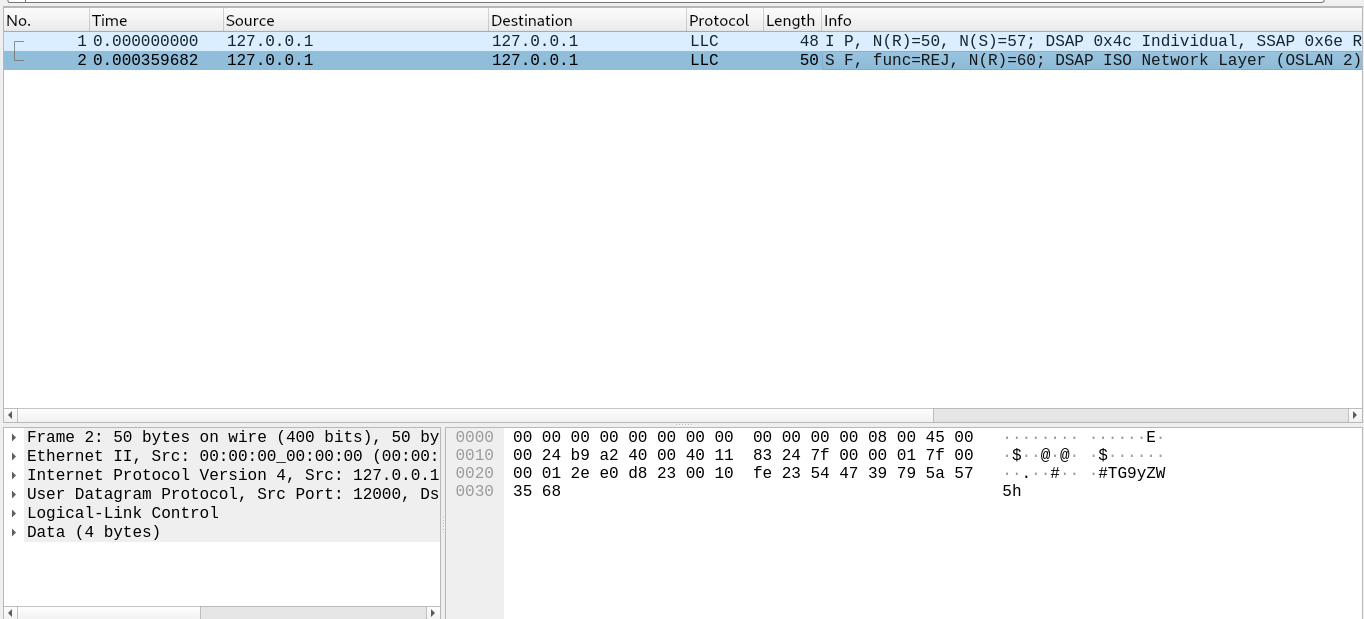
\includegraphics[width=0.7\textwidth]{assets/mensagemRecebidaB64.png} \end{center} As imagens evidenciam o caminho completo da mensagem: da entrada do usuário, passando pela codificação no servidor, até o retorno ao cliente. \section{Comando Netstat} A fim de comprovar o uso do protocolo de transporte e as portas de comunicação, foi executado o comando \texttt{netstat} durante a execução do experimento. A saída mostra a associação do processo Python à porta UDP 12000: \begin{center} 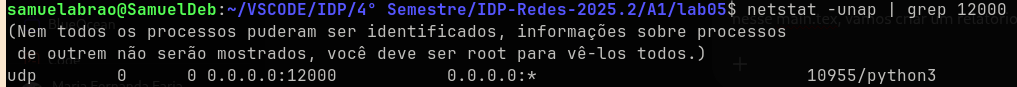
\includegraphics[width=0.8\textwidth]{assets/netstat.png} \end{center} O resultado demonstra que a porta de escuta está corretamente associada ao socket do servidor, e que o cliente realiza o envio de datagramas sem necessidade de conexão prévia. \section{Códigos Implementados} A seguir apresentamos os códigos completos utilizados no experimento. \subsection{Cliente (client.py)} \begin{lstlisting}[language=Python] from socket import * serverName = "127.0.0.1" serverPort = 12000 clientSocket = socket(AF_INET, SOCK_DGRAM) message = input("Digite sua mensagem: ") print(f"mensagem enviada {message}") clientSocket.sendto(message.encode(), (serverName, serverPort)) modifiedMessage, serverAddress = clientSocket.recvfrom(2048) print(f"mensagem recebida {modifiedMessage.decode()}") clientSocket.close() \end{lstlisting} \subsection{Servidor (server.py)} \begin{lstlisting}[language=Python] from socket import * import base64 serverPort = 12000 serverSocket = socket(AF_INET, SOCK_DGRAM) serverSocket.bind(("", serverPort)) print("Servidor pronto para recebimento de mensagens") while True: message, clientAddress = serverSocket.recvfrom(2048) print(message) modifiedMessage = base64.b64encode(message).decode() print(modifiedMessage) serverSocket.sendto(modifiedMessage.encode(), clientAddress) \end{lstlisting} \section{Discussão e Análise} O experimento demonstra a leveza e a praticidade da comunicação UDP. Observa-se que, mesmo sem garantias de entrega, a simplicidade do protocolo permite rápida transmissão de mensagens. Essa característica é desejável em cenários de tempo real, embora em aplicações críticas seja necessário aplicar camadas adicionais de confiabilidade. A utilização da codificação Base64 ilustra a importância da transformação de dados binários em formatos legíveis e seguros para transmissão. Na prática, o custo é um aumento de 33\% no tamanho da mensagem transmitida, mas em compensação garante compatibilidade com protocolos de transporte que podem não aceitar caracteres arbitrários. A captura do tráfego via \texttt{netstat} confirma a abertura da porta 12000 e o uso do UDP como protocolo de transporte. Ferramentas como Wireshark poderiam ainda revelar os pacotes em detalhe, evidenciando o payload correspondente às mensagens enviadas e recebidas. \section{Conclusão} O laboratório cumpriu os objetivos de introduzir os conceitos de programação com sockets, reforçar o entendimento sobre o protocolo UDP, e explorar a transformação de dados por meio de codificação Base64. Através da implementação prática, foi possível compreender como cliente e servidor trocam informações sem estabelecer uma conexão formal, além de verificar como os dados trafegam na rede. \end{document}